%\documentclass[aps,prl,groupedaddress]{revtex4-1}  % One column - tight
%\documentclass[aps,prl,preprint,groupedaddress]{revtex4-1}  % One column - spread
\documentclass[aps,prl,reprint,groupedaddress]{revtex4-1}  % Two column
%\documentclass[aps,prl,preprint,superscriptaddress]{revtex4-1}
%\documentclass[aps,prl,reprint,groupedaddress]{revtex4-1}

% Use the \preprint command to place your local institutional report
% number in the upper righthand corner of the title page in preprint mode.
% Multiple \preprint commands are allowed.
% Use the 'preprintnumbers' class option to override journal defaults
% to display numbers if necessary
%\preprint{}

% You should use BibTeX and apsrev.bst for references
% Choosing a journal automatically selects the correct APS
% BibTeX style file (bst file), so only uncomment the line
% below if necessary.
%\bibliographystyle{apsrev4-1}

% % % % % % % % % % % % Noam% % % % % % % % % % % % 
% Added preamble commands:
\usepackage[utf8]{inputenc}
\usepackage{array}
\usepackage{mathrsfs}
\usepackage{multirow}
\usepackage{amsmath}
\usepackage{graphicx}
\usepackage{float}  % For forcing a float position using 'H'.
\graphicspath{{../../figures/}}  % Search for graphics within the given directories.
\usepackage[unicode=true,pdfusetitle,bookmarks=true,bookmarksnumbered=false,bookmarksopen=false,
 breaklinks=false,pdfborder={0 0 1},backref=false,colorlinks=false]{hyperref}
%%%%%%%%%%%%%%%%%%%%%%%%%%%%%% User specified LaTeX commands.
\usepackage{braket}
\hypersetup{colorlinks=True,urlcolor=blue,linkcolor=blue,citecolor=blue,filecolor=black}
\usepackage[caption=false]{subfig}
% Extra commands
%\usepackage{lmodern}
%\usepackage[T1]{fontenc}
%\setcounter{secnumdepth}{3}
%\usepackage{color}
%\usepackage{float}
%\usepackage{mathtools}
%\usepackage{amssymb}
%\usepackage{breakurl}

%\usepackage{pslatex}  % Change font style.
%\renewcommand{\arraystretch}{1.5}  % Widens rows in Tables
%\setlength{\extrarowheight}{2pt}   % Widens rows in Tables

\makeatletter

\makeatother

\begin{document}

%Title of paper
\title{Final Project - TALENT 2017 at ECT* \\
		\small Structure of the Oxygen Isotopes}

% repeat the \author .. \affiliation  etc. as needed
% \email, \thanks, \homepage, \altaffiliation all apply to the current
% author. Explanatory text should go in the []'s, actual e-mail
% address or url should go in the {}'s for \email and \homepage.
% Please use the appropriate macro foreach each type of information

% \affiliation command applies to all authors since the last
% \affiliation command. The \affiliation command should follow the
% other information
% \affiliation can be followed by \email, \homepage, \thanks as well.
\author{T. Djärv, N. Gavrielov, L. Riz}
%\email[]{Your e-mail address}
%\homepage[]{Your web page}
%\thanks{}
%\altaffiliation{}
\affiliation{}

%Collaboration name if desired (requires use of superscriptaddress
%option in \documentclass). \noaffiliation is required (may also be
%used with the \author command).
%\collaboration can be followed by \email, \homepage, \thanks as well.
%\collaboration{}
%\noaffiliation

\date{\today}

\begin{abstract}
We examine the structure of $ ^{18-28} $O isotopes by employing our own shell-model program and by using the NushellX@MSU program. The former program is developed using the $ M $-scheme and is intended mainly for the $ sd $-shell, where an $ ^{16} $O core is assumed. Using our code we calculate energy spectra and occupation numbers and compare them with NushellX@MSU. Using NushellX@MSU we examine further observables such as (\textit{i}) the $ \beta $-decay of $ ^{22} $O to $ ^{22} $F, looking at the Fermi sum rule, $ q $-value and half-life of the decay, and (\textit{ii}) $ E2 $ transitions between the first $ 2^+ $ and the ground state using different interactions, for the even-even oxygen isotopes.
\end{abstract}

% insert suggested PACS numbers in braces on next line
\pacs{}
% insert suggested keywords - APS authors don't need to do this
%\keywords{}

%\maketitle must follow title, authors, abstract, \pacs, and \keywords
\maketitle

\newpage
\section{Introduction of our Theoretical Framework}
The oxygen isotopes have been widely investigated \citep[for a review see][]{Brown2017}. To describe their low lying spectrum within the shell model, different model spaces and interactions are used, starting from an $^{16}$O core with extra neutrons in the $sd$-shell \cite{Kuo1966,Wildenthal1984,Brown1988,Brown2006}, adding the lower $p$-shell for core-excitation (intruder states) with particle-hole configurations \cite{Lawson1976} and incorporating the $pf$-shell as well \cite{Utsuno1999}.

In this work we investigate the structure of the $^{18-28}$O isotopes, both even and odd, by examining their low-lying states. This is done by developing our own shell model program and comparing its results to the NushellX@MSU program \cite{Brown2014}.

We use an $^{16}$O core, having 8 protons and 8 neutron at the $s$-$p$-shells, ($0s_{1/2},0p_{3/2},0p_{1/2}$). 
More neutrons are then excited in the $sd$-shell ($0d_{5/2},1s_{1/2},0d_{3/2}$), which serves as our model space. We use all possible configurations in these orbits and work in a harmonic oscillator basis with spin-orbit splitting. 
The Hamiltonian reads

		\begin{equation} \label{eq:H}
		\hat H = \hat H_0 + \hat H_I,
		\end{equation}
for
		\begin{equation} \label{eq:H_0}
		\hat H_0 = \sum_{p} \epsilon_p \hat n_{p},
		\end{equation}
the one-body Hamiltonian, where $\hat n_p = \hat a_p^\dagger \hat a_p$ is the number operator for the spherical orbit $p$ with quantum numbers ($n_p,\ell_p,j_p,m_p$) and $\epsilon_p = \braket{p|h_0|p}$ are the single-particle energies (SPE). The interaction part reads
		\begin{equation} \label{eq:V}
		\hat H_I = \sum_{p < q=1}^{N} \sum_{r < s=1}^{N} V(p,q;r,s) \hat T(p,q;r,s),
		\end{equation}
		with
		\begin{equation} \label{eq:P}
		\hat T(p,q;r,s)  = \hat a_p^\dagger \hat a_q^\dagger \hat a_r \hat a_s,
		\end{equation}

$\hat H_I$ is given in $M$-scheme and is the two-body density operator for nucleon pairs in orbits $p,q$ and $r,s$ coupled to the total spin projection $M$, where $N$ is the number of particles in the configuration. In $J$-scheme $\hat H_I$ reads 
\begin{equation}
	\hat H_I =  \sum_{a\leq b,c \leq d} \sum_{JT} V_{J,T}(p,q;r,s) \hat T_{J,T}(p,q;r,s),
\end{equation}
where $\hat T_{J,T}(p,q;r,s)$ is the scalar two-body density operator for nucleon pairs in orbits $p,q$ and $r,s$ coupled to spin quantum numbers $J,M$ and isospin quantum numbers $T,T_z$ \cite{Brown2006}. Here the appropriate quantum numbers are $(n_i,\ell_i,j_i)$, $i \in \{a,b,c,d\}$. The transformation between the two-body matrix elements (TBME) from $J$- to $M$-scheme reads
\begin{multline}
	V(p,q;r,s)  =  \braket{j_{p},m_{p};j_{q},m_{q}|V|j_{r},m_{r};j_{s},m_{s}} \\ 
			    =  \mathcal{N}_{pq} \mathcal{N}_{rs} \sum_{J} \braket{j_{p},m_{p};j_{q},m_{q}|JM} \braket{j_{r},m_{r};j_{s},m_{s}|JM} \\
			   	\times \braket{(j_{p},j_{q})J||V||(j_{r},j_{s})J} \delta_{m_p+m_q,m_r+m_s},
\end{multline}
where other quantum numbers are implicitly implied. Here we have used the Wigner-Eckart theorem with the fact that $ V $ is a rank-zero tensor. Furthermore, $\braket{j_{a},m_{a};j_{b},m_{b}|JM}$ is a Clebsch-Gordan coefficient, $ \mathcal{N}_{pq} $ ($ \mathcal{N}_{rs} $) is a normalization factor and is equal $ \sqrt{2} $ if $ p=q $ ($ r=s $) with only even values of $ J $ and 1 if $ p \not=q $ ($ r \not=s $).

We use the SPE and TBME of the USDB interaction \cite{Brown2006} and work in $M$-scheme. The SPE values and order are given in Table \ref{tab:SPE}. The TBME for $A=18$ are given in \cite{Brown2006} in $J$-scheme for $T=1,0$ in Tables I and II, respectively. As was done for the USD interaction \cite{Wildenthal1984}, the SPE are taken to be mass independent and for the TBME we employ a mass dependence of the form
\begin{equation}
	V(p,q;r,s)(A) = \left( \frac{18}{A} \right)^p V(p,q;r,s)(A=18),
\end{equation}
with $p=0.3$. This qualitative mass dependence is expected from the evaluation of a medium-range interaction with harmonic-oscillator radial wave functions. It also defines TBME for other $A$ values in the $sd$-shell.

Using the single-particle states (SPS) we construct the appropriate slater determinants according to the number of particles which we place in the $sd$-shell. This enables us to construct expectation values of the Hamiltonian \eqref{eq:H} and diagonalize it to obtain the energies. 

In this work we represent a new shell-model code, compare it with NushellX results and conduct further investigation of the oxygen isotopes' wave functions using NushellX.

\begin{table}[H]
\caption{Single particle energies of the $sd$-shell in the $M$-scheme basis with their corresponding quantum numbers: $N$, the principle quantum number; $\ell$, the orbital angular momentum; $J$, the total angular momentum; $M_j$, the total angular momentum projection on the $z$ axis. \label{tab:SPE}}
\begin{ruledtabular}
\begin{tabular}{c|cccccc}
index	&	$N$	&	$\ell$	&	$J$	&	$M_j$	&	SPE			\\
\hline 
1		&	1	&	0		&	1	&	$-1/2$	&	-3.20790	\\
2		&	1	&	0		&	1	&	$+1/2$	&	-3.20790	\\
3		& 	0	&	2		&	3	&	$-3/2$	&	 2.11170	\\
4		&	0	&	2		&	3	&	$-1/2$	&	 2.11170	\\
5		&	0	&	2		&	3	&	$+1/2$	&	 2.11170	\\
6		&	0	&	2		&	3	&	$+3/2$	&	 2.11170	\\
7		&	0	&	2		&	5	&	$-5/2$	&	-3.92570	\\
8		&	0	&	2		&	5	&	$-3/2$	&	-3.92570	\\
9		&	0	&	2		&	5	&	$-1/2$	&	-3.92570	\\
10		&	0	&	2		&	5	&	$+1/2$	&	-3.92570	\\
11		&	0	&	2		&	5	&	$+3/2$	&	-3.92570	\\
12		&	0	&	2		&	5	&	$+5/2$	&	-3.92570	
\end{tabular}
\end{ruledtabular}
\end{table}
\section{LNLT\_shell} \label{sec:CodeExpl}
% General Introduction about the shell model code
%% Toy code, with goal to compute oxygen isotope spectrum in the sd shell

Throughout this project a simple shell-model code, called ``LNLT\_shell'', has been developed in python. The main goal of this shell-model is to be able reproduce the oxygen isotopes spectra in the sd-shell.

A nuclear shell-model code approximates the spectrum for an atomic Nucleus with \(A\) nucleons by assuming a frozen core with \(A_{\rm{core}}\) nucleons, and then solves the many-body Schrödinger equation \(H\ket{\Psi}=E\ket{\Psi}\) where \(H\) is described in equation \ref{eq:H}
for a group of \(n=A-A_{\rm{core}}\) valence nucleons.


% The general structure
%% Parse arguments (more about what arguments that exist rather that how)

The program starts by parsing the argument list. There are six different arguments:
\begin{itemize}
\item[-n n:] Used to specify number of valence nucleons.
\item[-M M:] Used for total-M restriction, discussed below.
\item[-of filename:] To specify what json file contains the shells.
\item[-os bool:] To turn the pairing basis on and off.
\item[-if filename:] To specify what file contains the two-body matrix elements.
\item[-o filename:] To specify what file to write the output to.
\item[-nu directory:] To specify where the NuShellX results are located for the target nucleus.
\end{itemize}
observe that -of and -if are mutually exclusive.


%% Reading/setting up the shells and single particle basis


The first thing the code does after parsing the arguments is setting up the single particle basis.
This is done either by reading them directly from the m-scheme matrix element file %\cite Morten and Alex
or by constructing them from shells it reads in a given json file.

% Format n l 2j 2m ?

%% Setting up all possible Slater Determinants

When the single particle basis is determined, all possible Slater determinants for the valence nucleons are constructed to form the many-body basis.
This is done by constructing all unique combinations of \(n\) single particle states, each such combination representing a Slater determinant.
%% M-Restriction
After the many-body basis is constructed, it is possible to apply total M-restriction to exploit that the used Hamiltonian is a spherical scalar and therefore block-diagonal in total \(M\). This is done by removing all Slater determinants that do not have the desired total \(M\).

%% Discuss the TwoBodyOperator class, not go in to detail but the general ideas
The many-body Hamiltonian matrix is constructed in the class TwoBodyOperator, by acting with \(\bra{a,b}V\ket{c,d}_{AS}a^\dagger_a a^\dagger_b a_d a_c\) repeatedly for different values of \(a,\,b,\,c,\,d\) on all the Slater determinants in the many-body basis to determine which states differ with up to two single-particles states. This process results in a full matrix
%% The diagonalisation using numpy
which then is diagonalized by applying a full diagonalization routine from numpy. % cite numpy?
This results in list of eigen energies \(E\) with associated eigen states \(\ket{E,i}\) where \(i\) takes in to account potential degeneracy.

%% The J^2 operator
When the eigenstates to the Hamiltonian has been computed, the total angular momentum of each state is computed by solving  \(\hbar^2 J(J+1) = \bra{E,i}\hat{J}^2\ket{E,i}\) for each state. The operator \(\hat{J}^2\) can be divided in a two- and one-body operator, from which a many-body matrix can be obtained with the same machinery described for the full Hamiltonian matrix.

%% Occupation numbers
For each state shell-occupation number is determined by the application of
\begin{equation}
  \bra{E,i}n_k\ket{E,i}=\bra{E,i}\sum_{m=-j}^j a^\dagger_{k,m}a_{k,m}\ket{E,i}
\end{equation}
where \(k\) represents the shell, and \(j\) is associated to shell \(k\).

%% The output format
The program writes the results to the screen and optionally to a user specified file, where the single-particle basis, the many-body basis, the eigen-spectrum of the Hamiltonian and the shell-occupation numbers can be seen.

Different interactions can be provided in two different ways. Either by a file which format will be described below, or as a class containing a method get\_matrix\_element that takes four single particle states as its arguments.
The matrix element file starts by stating how many single-particle states there are, and then continues listing them together with the single-particle energies. There after the file contains a number \(l\) representing how many two-body matrix elements there exists, followed by \(l\) lines of four integers representing the two-body states on the bra and ket side of the two-body matrix element and one fixed point value with \(5\) decimals and one hole number.

\section{Comparision between LNLT\_shell and NuShellX}
% Displaying the eigne values of each program side by side.
% comment on that we compute more states than nushellx computes.
% display the occupation numbers

To verify that the code described in the previous section works, several isotopes of oxygen were computed with LNLT\_shell and compared to the result from NuShellX with the USDB interaction. In Table \ref{tab:ox18},\ref{tab:ox19} and \ref{tab:ox20} the eigenenergies of \(^{18,19,20}\rm{O}\) are compared to the values computed with NuShellX. The energies are relative the ground energy of \(^{16}\rm{O}\). There are almost no difference to the given numerical precission, only a few of the higher eigen-values differ slightly. In addition the code seems to correctly assign total angular momentum; the \(J_L\) columns are identical with the \(J_N\) columns. To illustrate the similarity further, the lowest energies are plotted in Fig. \ref{fig:ox18eig},\ref{fig:ox19eig} and \ref{fig:ox20eig}, where also a comparision to experiment is made.

\onecolumngrid

\begin{figure}[h!]
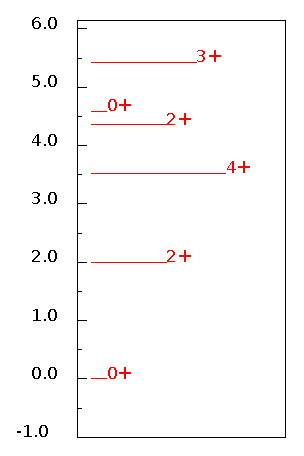
\includegraphics{ox18.eps}
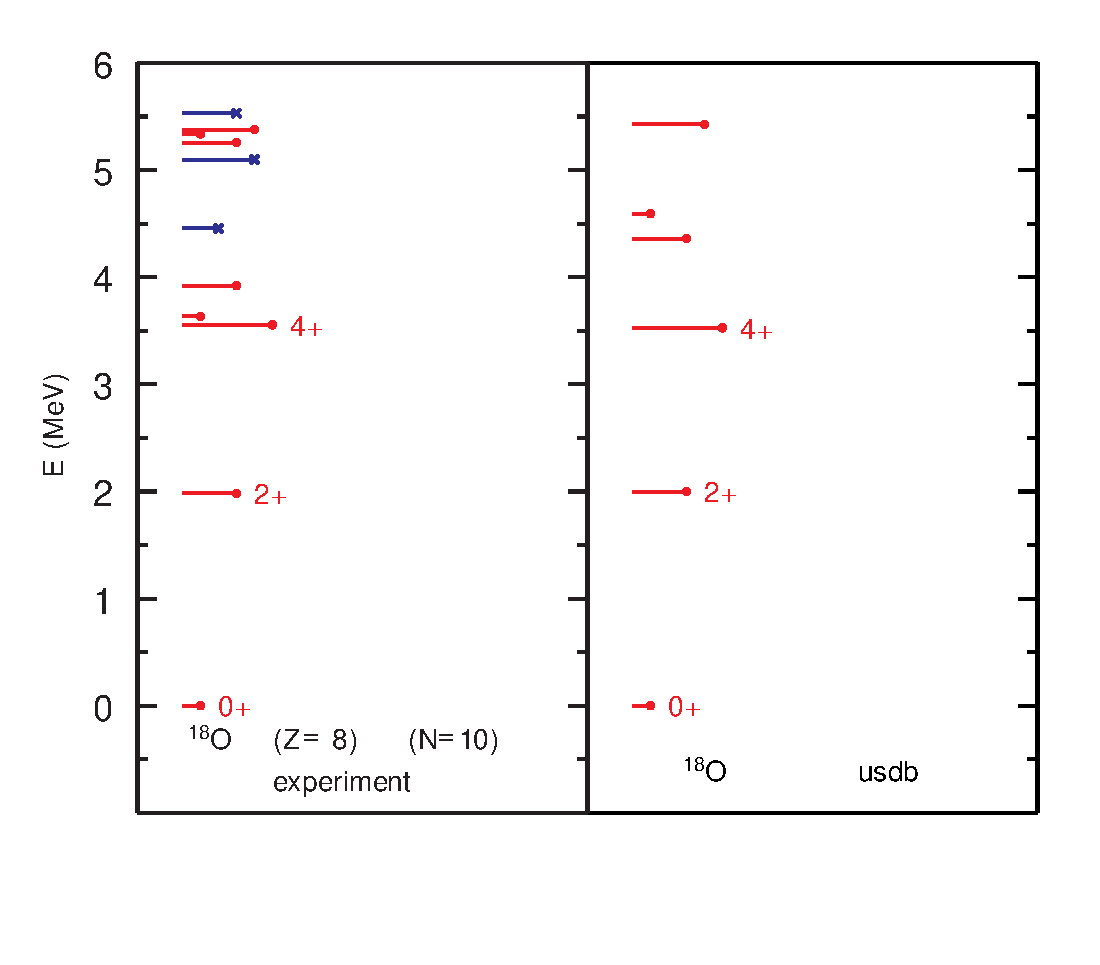
\includegraphics[scale=0.56,trim=0cm 2.3cm 0cm 0cm]{o_18b.eps}
\caption{The lowest energy states of $^{18}\rm{O}$, computed by LNLT\_shell to the left compared to the eigenspectrum from experiment and NuShellX to the right}
\label{fig:ox18eig}
\end{figure}

\begin{figure}[h!]
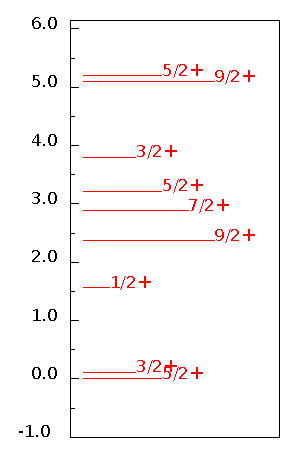
\includegraphics{ox19.eps}
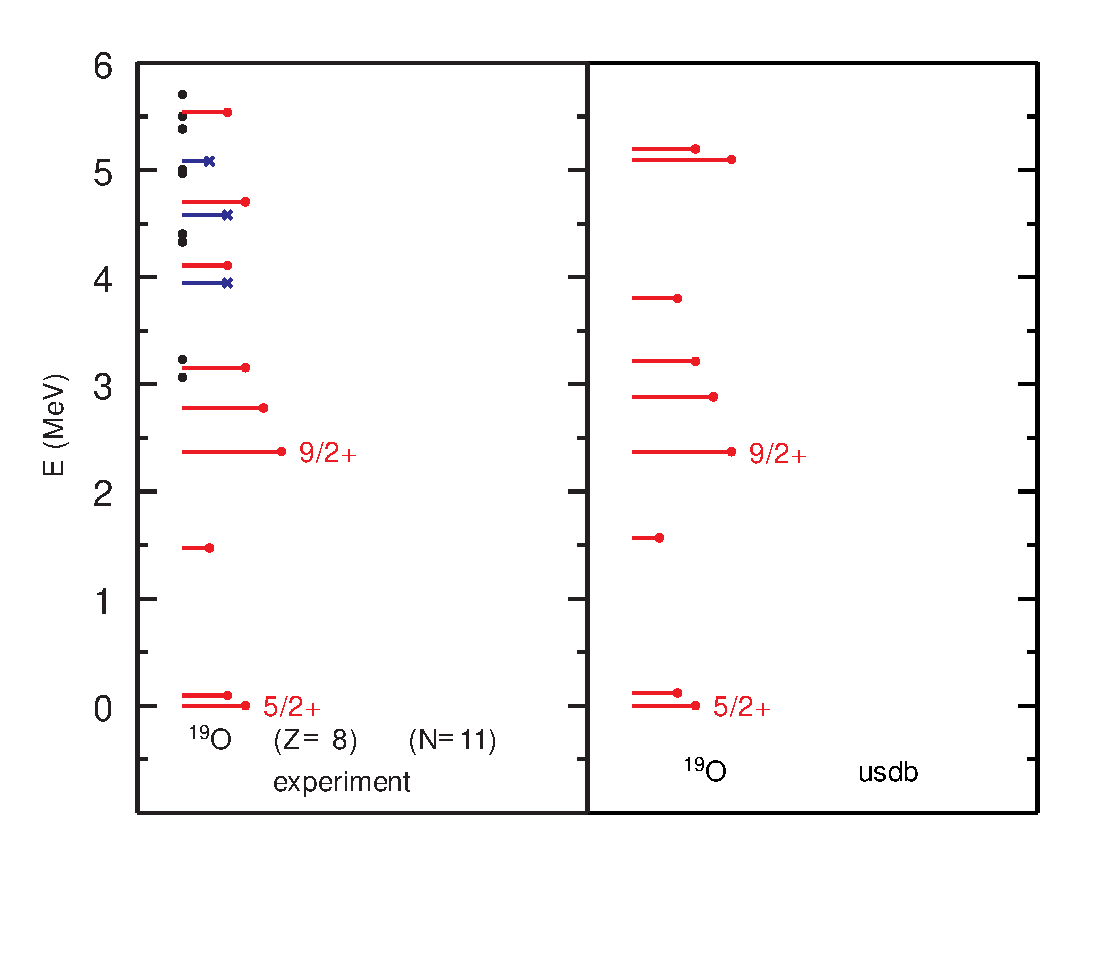
\includegraphics[scale=0.56,trim=0cm 2.3cm 0cm 0cm]{o_19b.eps}
\caption{The lowest energy states of $^{19}\rm{O}$, computed by LNLT\_shell to the left compared to the eigenspectrum from experiment and NuShellX to the right}
\label{fig:ox19eig}
\end{figure}

\begin{figure}[H]
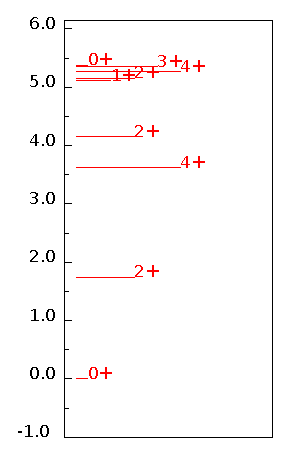
\includegraphics{ox20.eps}
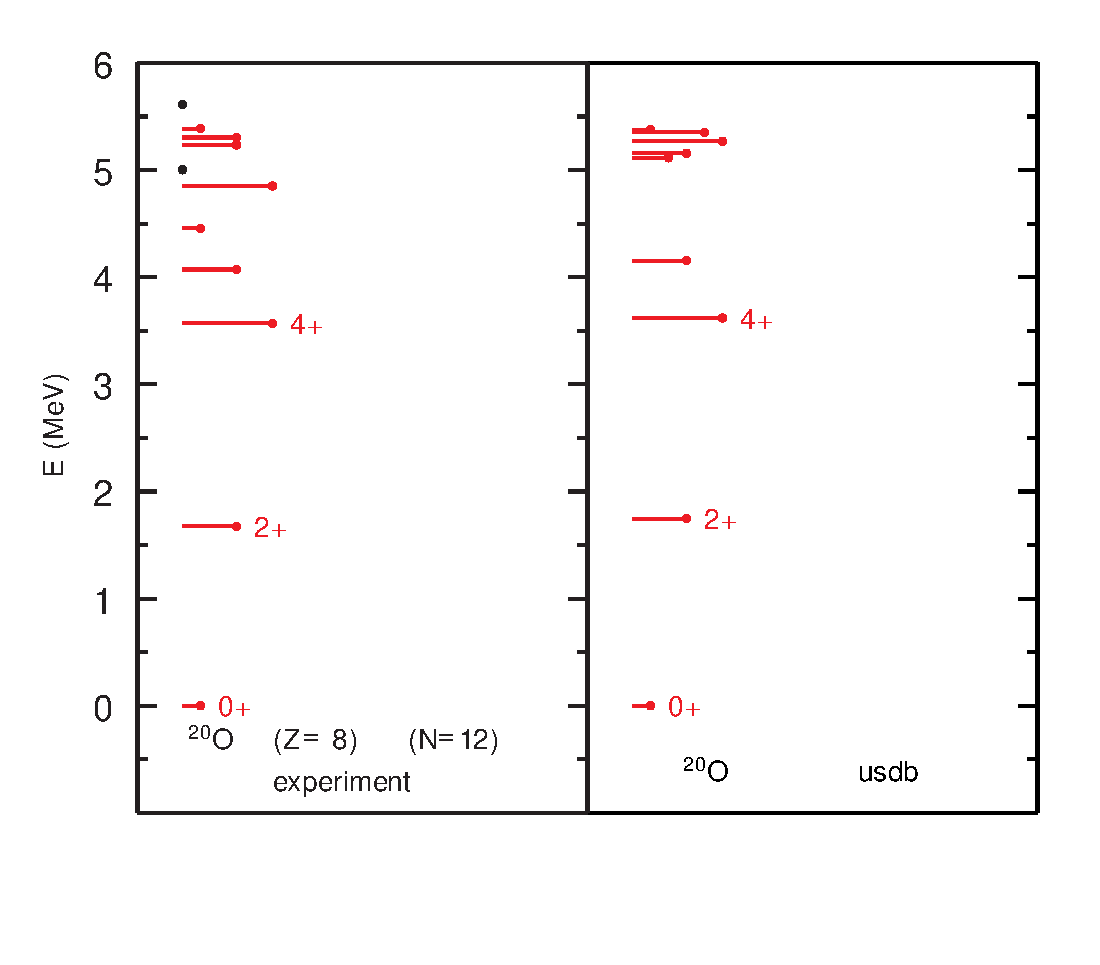
\includegraphics[scale=0.56,trim=0cm 2.3cm 0cm 0cm]{o_20b.eps}
\caption{The lowest energy states of $^{20}\rm{O}$, computed by LNLT\_shell to the left compared to the eigenspectrum from experiment and NuShellX to the right}
\label{fig:ox20eig}
\end{figure}

\twocolumngrid

In addition to the eigen-spectrum for each isotope shell-occupation numbers were also computed. In Table \ref{tab:ox18occ} all the shell-occupation numbers for all \(14\) states can be viewed, computed both with LNLT\_shell and with NuShellX. There are some slight difference, however this can be easily explained with that LNLT\_shell outputs higher precision than NuShellX does and thus the difference is most likely due to rounding errors. In Figs. \ref{fig:occnum_lnlt} and \ref{fig:occnum_nushellx} the shell occupation for the ground state and the first excited states are visualized, computed by LNLT\_shell and NuShellX respectively. Also here there are a slight differences, which still can be explained with rounding errors. \\

\onecolumngrid

\begin{figure}[H]
  \begin{center}
  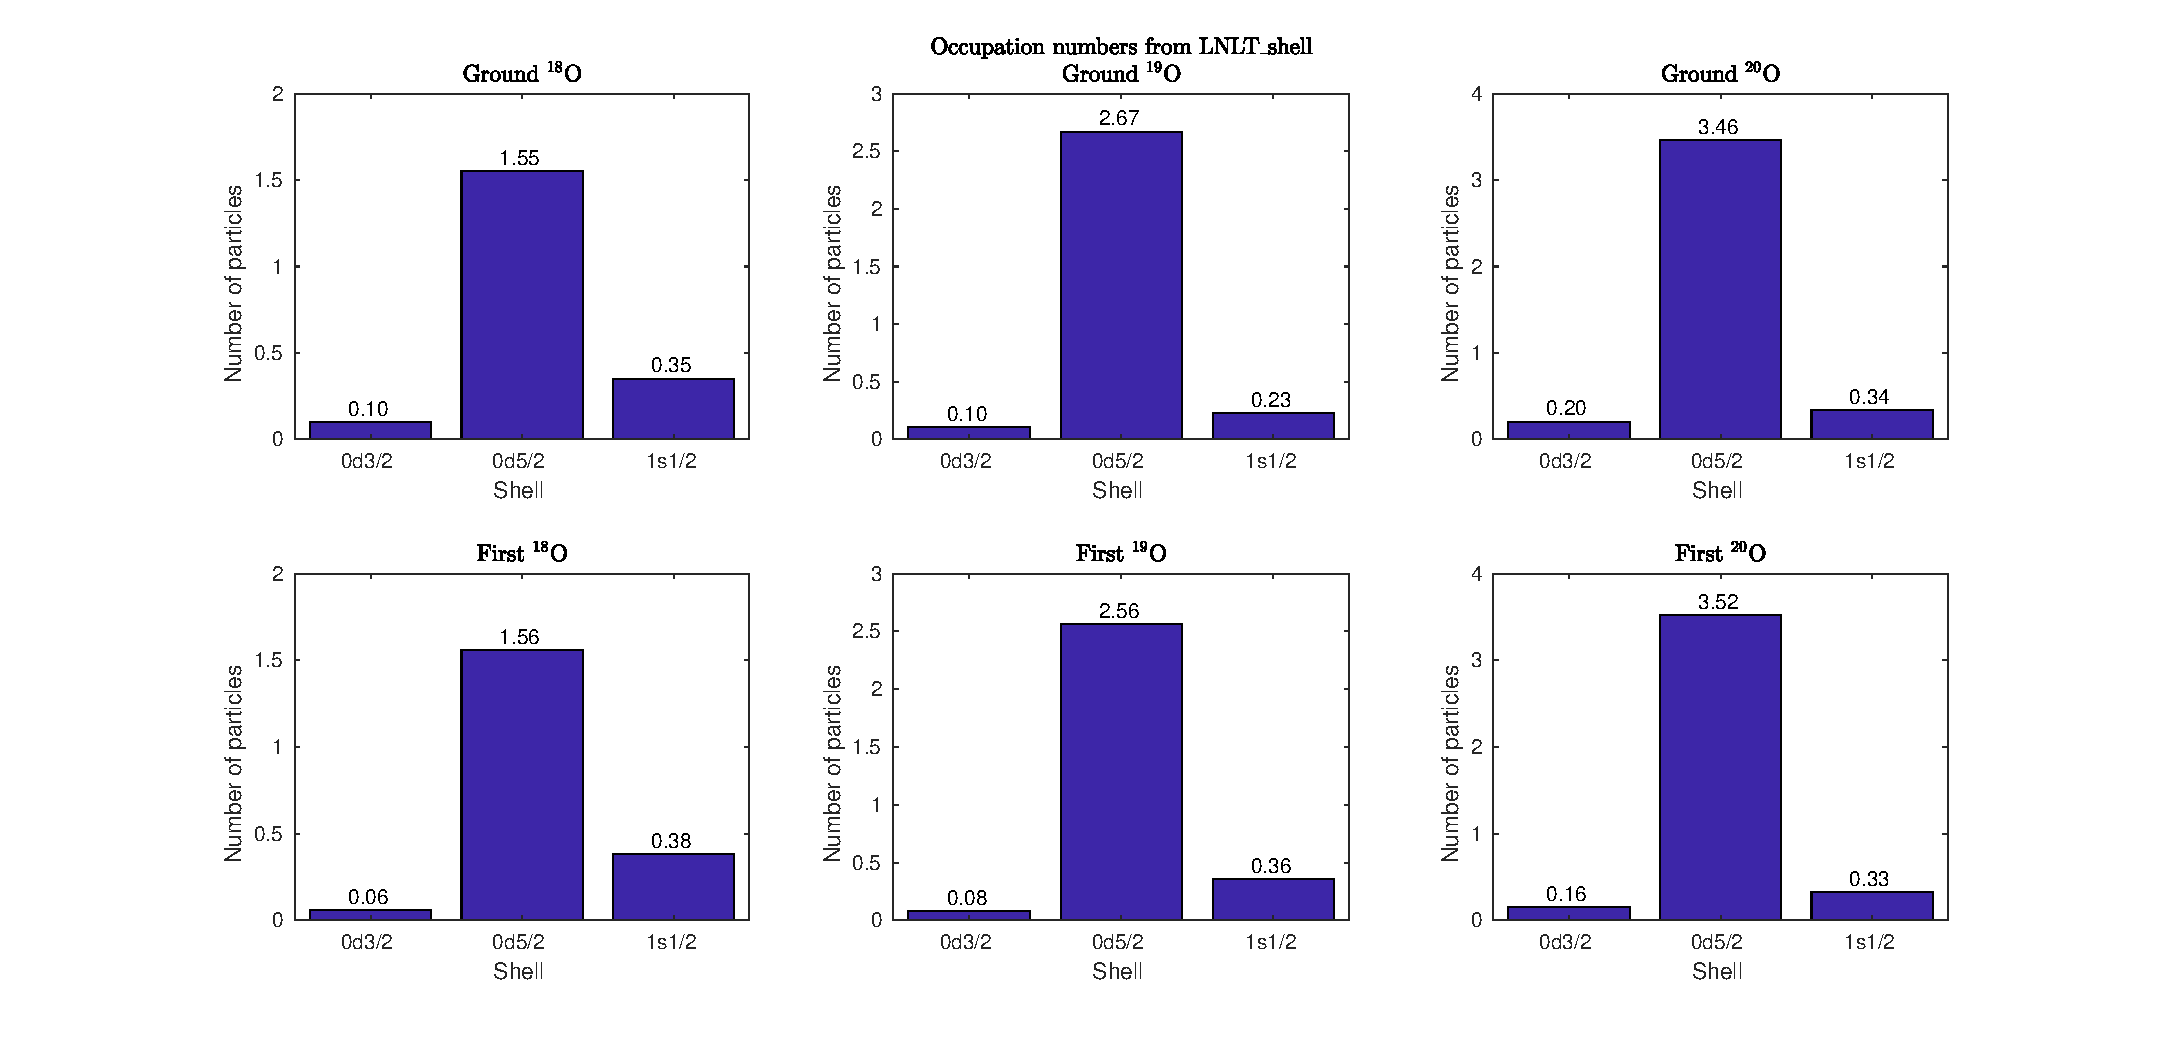
\includegraphics[scale=0.5]{occupation_numbers_lnlt.eps}
  \caption{The occupation numbers of the ground state and first excited state of \(^{18,19,20}\rm{O}\) as computed by LNLT\_shell.}
  \label{fig:occnum_lnlt}
  \end{center}
\end{figure}

\begin{figure}[H]
  \begin{center}
  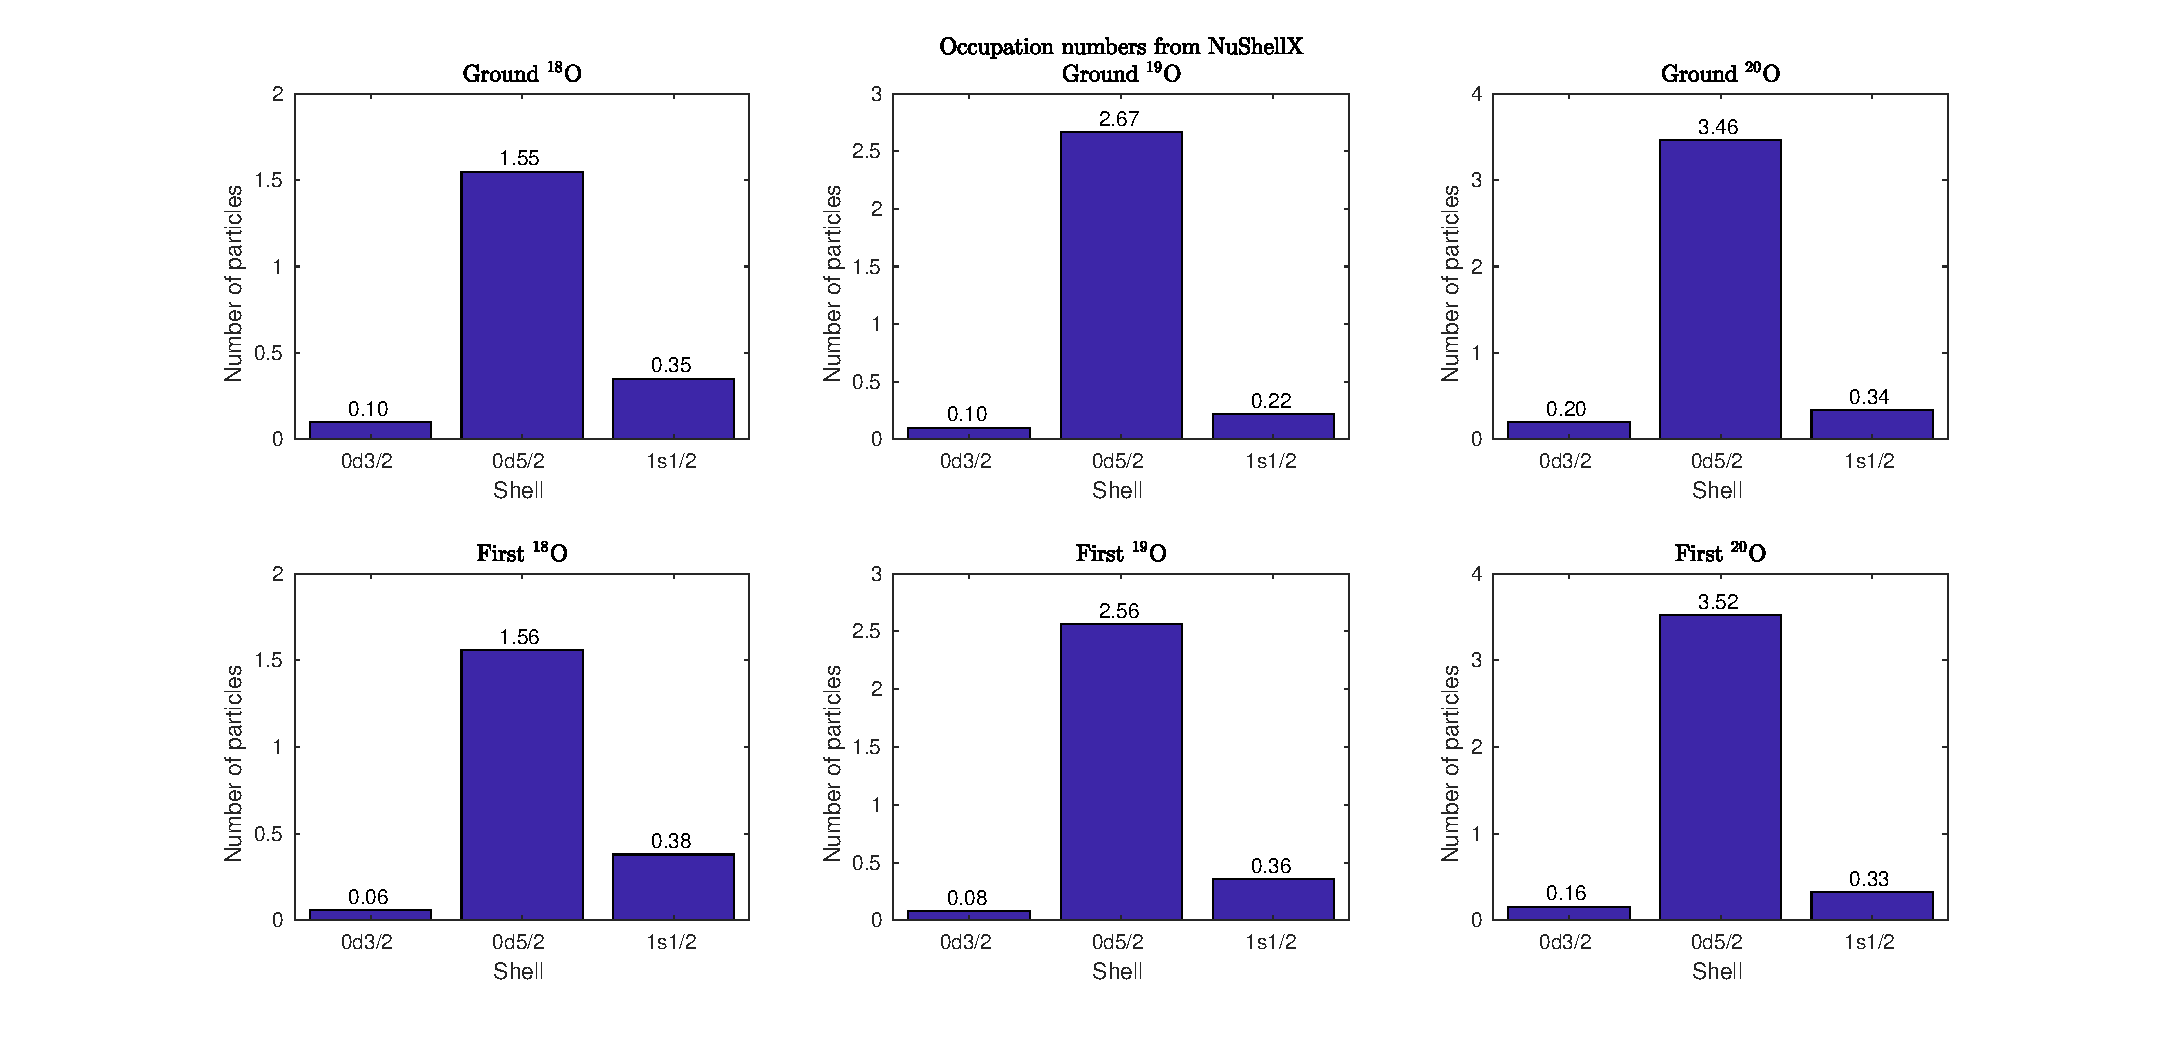
\includegraphics[scale=0.5]{occupation_numbers_nushellx.eps}
  \caption{The occupation numbers of the ground state and first excited state of \(^{18,19,20}\rm{O}\) as computed by NuShellX.}
  \label{fig:occnum_nushellx}
  \end{center}
\end{figure}

\twocolumngrid

\section{NushellX}
The structure of the wave functions of different levels in the oxygen isotopes is interesting to examine since it can reveal the role of different configurations and orbits. Furthermore, within a given configuration examining different interactions using different observables can be also insightful. 
In the first subsection we examine using NushellX@MSU the spectra of oxygen isotopes and the capability of different interactions, the USDA, USDB and coupled cluster effective interaction (CCEI) \cite{Jansen2016} to reproduce spectra. The second subsection is devoted to the study of Fermi and Gamow-Teller $\beta$-decay of $^{22}$O and how the USDB and CCEI interactions fulfill sum rules. The third subsection address electromagnetic transitions rates for different isotopes and interactions.

\subsection{Oxygen isotopes spectra with different interactions} \label{Oxygen}
%
We analyze how the different interactions reproduce the excitation energy of the first $2^+$ state in even-even oxygen isotopes from $^{18}$O to $^{26}$O and compare to experiment. This is seen in Fig. \ref{fig:2+/0+}   and gives an indication on the location of the shell closure. The latter  arises when the excitation energy from the g.s. to the first excited $2^+$ state is at maximum.

\begin{figure}[htb!]
\centering
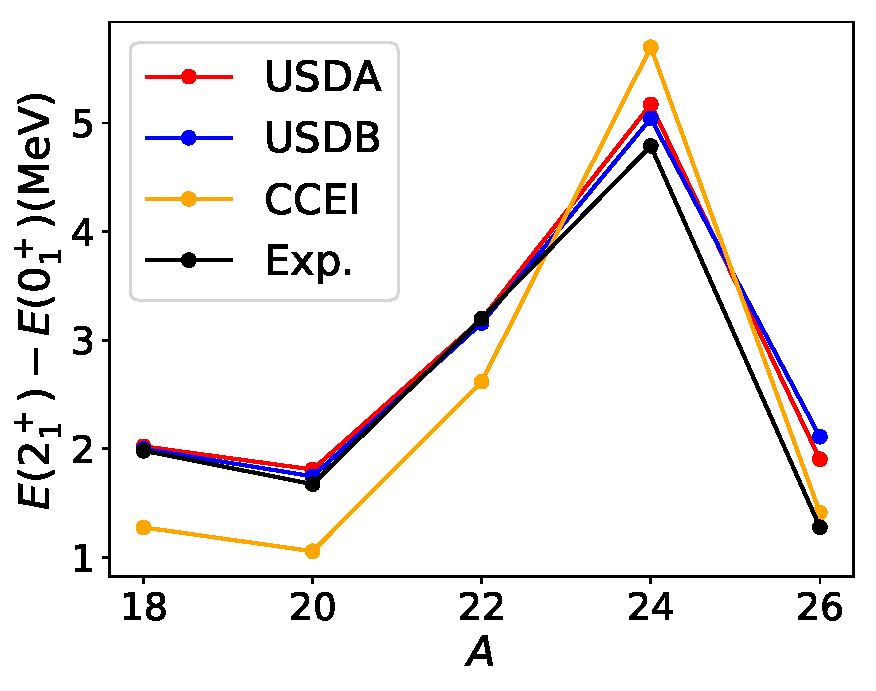
\includegraphics[width=1\linewidth]{2+_over_0+.pdf}
\caption{Excitation energy of the first $2^+$ state in oxygen isotopes (even-even). Experimental errorbars are really small compared to plot resolution.}
\label{fig:2+/0+}
\end{figure}

The USDA and USDB interactions give similar results,  are in good agreement with experimental results and give a good description of the shell closure at $^{24}$O. Since USDB has more linear combination of parameters than USDA it generates a better agreement with the experimental results. 
The CCEI interaction underestimates the excitation energies up to $^{26}$O, while at shell closure it emphasize this effect by overestimating the first $2^+$ state energy. 
It is interesting to note that CCEI interactions seems to give a good description in rich neutron isotopes, close to the neutron drip line. This may be due to the presence of Coulomb forces CCEI interaction and are therefore iso-spin breaking and it behaves differently with increasing neutron number in isotope chains.

We next explore the spectra of even-odd oxygen isotopes. Among them we analyze the spectrum of $^{19}$O since it has the largest amount of experimental data. The results are shown in Fig. \ref{fig:19O}. Note that the experimental results show also negative parity states (blue lines), which are not included in our theoretical calculations since we are working in the $sd$ model space. For completeness black dots in the experimental panel indicate states which have not been assigned to a definite parity.

\onecolumngrid

\begin{figure}[htb!]
\centering
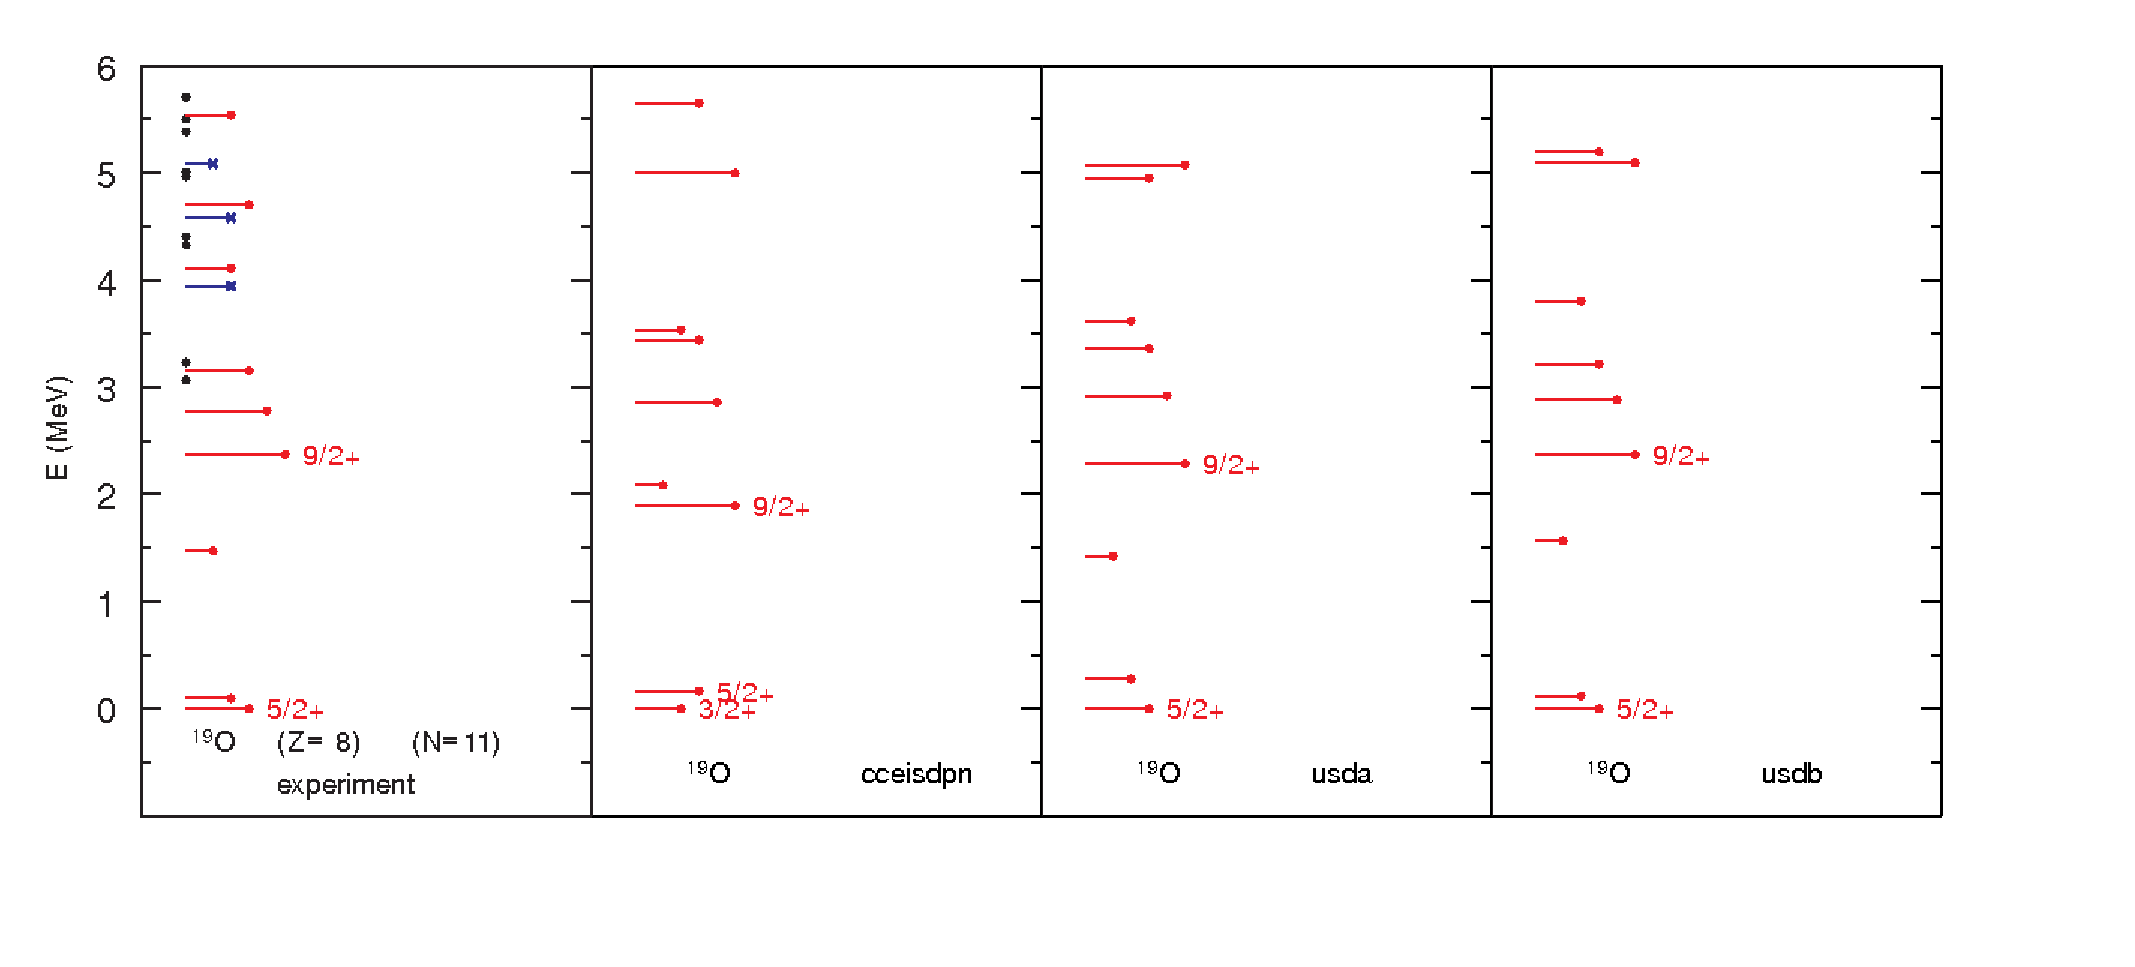
\includegraphics[width=\textwidth]{19O.eps}
\caption{$^{19}$O spectrum with different interactions compared to experiments.}
\label{fig:19O}
\end{figure}

\twocolumngrid

The USDA and USDB reproduce the correct spin orderings, where the USDA yields better results up to the first $1/2^+$ at energy 1.422 MeV and the USDB yields better results from the first $9/2^+$ at energy 2.370 MeV up to the second $3/2^+$ at energy 3.802 MeV. The differences are not significant though and further tests for comparison could be electromagnetic transition rates.
The CCEI exchanges the order of the first $3/2^+$ with the g.s. and the order of the first $9/2^+$ and the first $1/2^+$, causing both pairs to be nearly degenerate. The former case is reasonable since the g.s. and the first $3/2^+$ are nearly degenerate,  however the latter case exhibits a larger discrepancy from experiment. This different level ordering may also be related to the inclusion of Coulomb forces in CCEI interaction, which may exchange energy-levels.

%
\subsection{Fermi and Gamow-Teller $\beta$-decay of $^{22}$O}
%
On top of energies, it is insightful to examine other observables in order to understand better the differences between different interactions. We analyze the $\beta$-decay of $^{22}$O to $^{22}$F.
We perform the calculations using NushellX for the USDB and CCEI interactions (USDA interaction gives similar results of USDB interaction). 
\begin{table}[h!]
\caption{Sum Rules}
\begin{center}
\begin{tabular}{l@{\qquad}l@{\qquad}r@{\qquad}rl}
\hline
\multicolumn{1}{l}{\rule{0pt}{12pt}
                   }&\multicolumn{1}{l}{\rule{0pt}{12pt} sum rule}&\multicolumn{1}{l}{CCEI}&\multicolumn{2}{l}{USDB}\\[2pt]
\hline\rule{0pt}{12pt}
sum b(f)            &  $N_i-Z_i=6$   & 5.9993 & 6.0000 &\\
sum qf$\cdot$b(gt)  &  $\ge 3\cdot(N_i-Z_i)=18$  & 6.0346 & 10.0335 &\\[2pt]
\hline
\end{tabular}
\end{center}
\end{table}

Both interactions fulfill the theoretical Fermi sum rule, but in different ways.
The contribution of the CCEI interaction to the Fermi sum rule b(f) splits among different states: this is because the e interaction has several nearly degenerate levels which mix. The USDB interaction gives all the contribution to b(f) in one single state, which is the isobar analogue of the $^{22}$O.

Let us compare the results obtained with the two different interactions to the experimental results for the q-value and the half-life. Note that one has to include more than only the default ten levels for each spin state in NushellX in order to get significant results, otherwise too much information is neglected.
\begin{table}[h!]
\caption{q-value and t$_{1/2}$}
\begin{center}
\begin{tabular}{r@{\qquad}r@{\qquad}r@{\qquad}r@{\qquad}l}
\hline
\multicolumn{1}{l}{\rule{0pt}{12pt}
                   }&\multicolumn{1}{l}{exp}&\multicolumn{1}{l}{CCEI}&\multicolumn{2}{l}{USDB}\\[2pt]
\hline\rule{0pt}{12pt}
q-value [MeV]   &     6.489 & 6.847 & 8.437 &\\
t$_{1/2}$ [sec] &     2.25  & 0.478 & 2.620 &\\[2pt]
\hline
\end{tabular}
\end{center}
\end{table}

The CCEI interaction gives a good description of the q-value, but underestimates the half-life, while the USDB interaction is in good agreement with the experimental value for the half-life, but slightly overestimates the q-value.

\subsection{$ E2 $ transitions of the oxygen isotopes}
Here we will only investigate the $E2$ between the first $2^+$ and the first $0^+$, i.e. $B(E2; 2_1^+ \rightarrow 0_1^+)$, using the USDA, USDB and CCEI interactions, given in Fig. \ref{oxygen-be2}. For the experimental data there are only three values, however it is notable that they become closer to the theoretical values as neutrons are added, with the largest discrepancy occurring for the $^{18}$O isotope. The reason might be due to the fact we are neglecting $p$-shell core-excitations when using only the $sd$-shel model space. It was found in \cite{Lawson1976} that the $0_2^+$ should have a dominant $4p-2h$ component. However there are indications that mixing should arise, and perhaps with the $0_1^+$. As for the $2^+_1$, there might be less mixing with an intruder configuration since the $2^+_3$, which has a large intruder component, is high in energy (5.255 MeV) 	 and thus mixes less with the $2^+_1$. The problem for mixing of these states due to the truncation in the $np–mh$ sequence is discussed in \cite{Warburton1992a}. Therefore, when close to the $^{16}$O core, e.g. at $^{18}$O, a some part of the $p$-shell is missing in the wave function of $0^+_1$ rendering less components in the wave functions to connect between the $0_1^+$ and the $2_1^+$ and hence yielding a smaller $B(E2)$ value. As neutrons are added to the $^{16} $O core, the $p$-shell core-excitations move to higher energy and mix less with the low-lying states, then the $sd$-shell model space becomes a better approximation. As seen in Fig. \ref{oxygen-be2}, this is correct for all three interactions which operate in the $sd$-shell. Although the CCEI does not reproduce energies as well as USDA and USDB, it gives a slightly better approximation for the $B(E2; 2_1^+ \rightarrow 0_1^+)$. Yet, the differences are minor and other observables should be examined.

\begin{figure}[h]
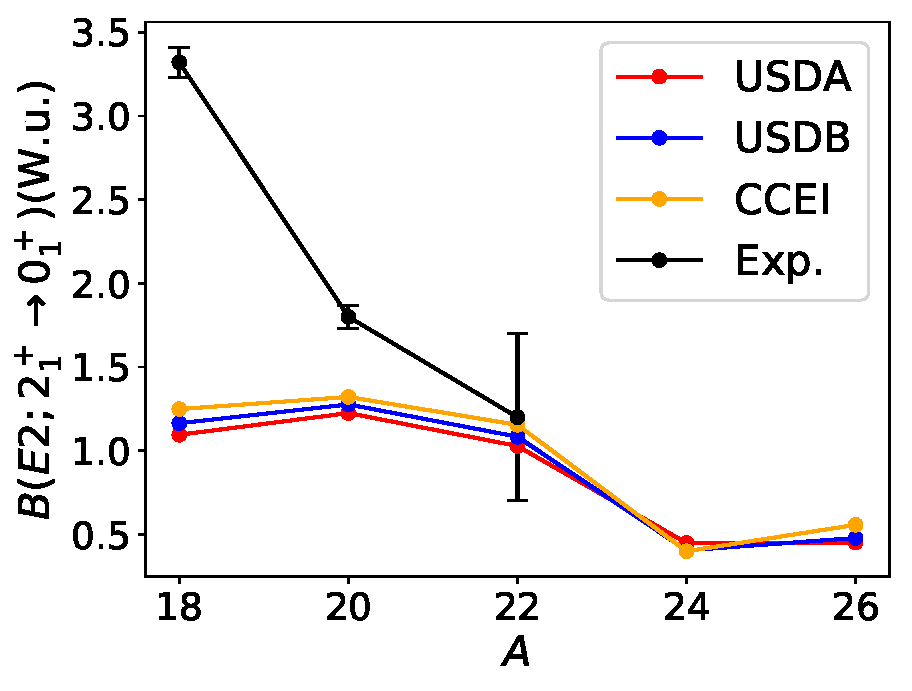
\includegraphics[width=1\linewidth]{../figures/oxygen-be2.pdf}
\caption{$B(E2; 2^+ \rightarrow 0^+)$ of experimental (black), the USDA (red), USDB (blue) and CCEI (orange) interactions for $^{18-26}$O. \label{oxygen-be2}}
\end{figure}



\section{Conclusions and Outlook} \label{sec:conclusions-and-outlook}

We succesfully develop a simple shell-model code, which is able to reproduce the results obtained with the already enstablished NushellX code,  with the same interaction(USDB), but working in $M$-scheme.
The code we develop is able to describe all oxygen isotopes within the $sd$-model space and to give prediction on their spectra. Moreovere we were able to implement the computation of operators such as occupation number and $J^2$ in our code.
It is important to remark that the performace of our code is worse than the professional code NushellX, but the main aim was to be able to self-develop a simple shell-model code.

On the other side we examine using NushellX the spectra of oxygen isotopes, looking at the effect of different interactions (USDA, USDB and CCEI).
We explored and analysed not only spectra of oxygen isotopes, but we look also at the effect of different interaction in the study of Fermi and Gamow-Teller $\beta$-decay of $^{22}$O and electromagnetic transitions rates in different oxygen isotopes.
While USDB and USDA interactions give really similar results with respect to all the observables we studied, the CCEI interaction shows interesting deviations from USD-type interactions behavior.
This is mainly due to the presence of the Coulomb interaction, which breaks isopin, and mixes up states differently from USD-type interactions.

There are many things that can be improved with the toy shell-model code presented in this work. The code presented in this work are slow and only practically applicable on small model spaces. Further at the moment it can only use the usdb interaction. This is a problem since different interactions could be necessary to include. The current code is tailored to only work with neutrons as valence nucleons, this makes it only possible to study a limited set of nuclei. When comparing theory to experiment it might be beneficial to study different observables, in the present condition our code can compute besides the eigenspectrum, total angular momentum and occupation numbers, but there are many others interesting observables that could be of interest both to theoreticians and experimentalists.

That first issue that we would like to tackle if we are to continue this project is that of speed.
Currently our code uses an exact eigenvalue solver imported from numpy, which works fine for small models spaces. However, for larger model spaces iterative algorithms such as Lanczos is a better option. Some work on this has already been done, however we never finished it.

To further increase speed of shell-model codes, an interesting approach is to use the similarity between number-representation of Slater-determinants and binary numbers, and that most computers today uses binary numbers internally. We have been looking in to this and a skeleton of a shell-model code using this approach has been partially written in C++.

The next step of hypothetical improvements would be to allow for valence protons as well as the currently implemented valence neutrons. For the pure proton-proton part of such an improvement the same technology as for the already implemented neutron-neutron case can be used, so the only hard addition would be to implement the proton-neutron interactions.

Further improvements could involve implementation of spectroscopic factors. Since a lot of interesting nuclear physics involves nuclear decay this is a given improvement. Some attempts has been made already to do this, for the removal of neutrons. Unfortunately the authors underestimated the time it would take to make this work.



\newpage
\appendix
\onecolumngrid
\section{Tables}

\begin{table}[H]
\centering
\caption{The energy spectrum of $^{18}\rm{O}$ computed with LNLT\_shell (to the left) compared to NuShellX result (to the right). \(J_L\) is computed with LNLT\_shell while \(J_N\) are computed with NuShellX.}
\label{tab:ox18}
\begin{tabular}{c|cc|cc}
\hline Nr & \(E\) & \(J_{L}\) & \(E_{\rm{NuShellX}}\) & \(J_{N}\) \\
\hline 1   & -11.932 &       0 & -11.932 & 0 \\
 2   &  -9.933 &       2 & -9.933 & 2 \\
 3   &  -8.405 &       4 & -8.405 & 4 \\
 4   &  -7.572 &       2 & -7.572 & 2 \\
 5   &  -7.339 &       0 & -7.339 & 0 \\
 6   &  -6.505 &       3 & -6.505 & 3 \\
 7   &  -2.912 &       4 & -2.912 & 4 \\
 8   &  -2.051 &       2 & -2.050 & 2 \\
 9   &  -1.162 &       1 & -1.162 & 1 \\
 10  &  -0.991 &       3 & -0.991 & 3 \\
 11  &  -0.901 &       2 & -0.901 & 2 \\
 12  &  -0.577 &       1 & -0.577 & 1 \\
 13  &   3.077 &       0 & 3.077 & 0 \\
 14  &   4.288 &       2 & 4.288 & 2 \\
\hline
\end{tabular}
\end{table}

\begin{table}[h]
\caption{The energy spectrum of $^{19}\rm{O}$ computed with LNLT\_shell (to the left) compared to NuShellX result (to the right). \(J_L\) is computed with LNLT\_shell while \(J_N\) are computed with NuShellX.}
\label{tab:ox19}
\begin{tabular}{c|cc|cc||c|cc|cc}
\hline Nr & \(E\) & \(J_{L}\) & \(E_{\rm{NuShellX}}\) & \(J_{N}\) & Nr & \(E\) & \(J_{L}\) & \(E_{\rm{NuShellX}}\) & \(J_{N}\) \\
\hline 1   & -15.956 &       5/2 & -15.956 & 5/2 & 20  &  -5.247 &       9/2 & -5.247 & 9/2 \\
 2   & -15.838 &       3/2 & -15.838 & 3/2 & 21  &  -5.211 &       7/2 & -5.211 & 7/2 \\
 3   & -14.389 &       1/2 & -14.389 & 1/2 & 22  &  -5.155 &       5/2 & -5.155 & 5/2 \\
 4   & -13.586 &       9/2 & -13.586 & 9/2 & 23  &  -4.713 &       1/2 & -4.713 & 1/2 \\
 5   & -13.072 &       7/2 & -13.072 & 7/2 & 24  &  -4.676 &       3/2 & -4.676 & 3/2 \\
 6   &  -12.74 &       5/2 & -12.740 & 5/2 & 25  &  -4.001 &       5/2 & -4.002 & 5/2 \\
 7   & -12.153 &       3/2 & -12.153 & 3/2 & 26  &  -3.379 &       3/2 & -3.379 & 3/2 \\
 8   & -10.859 &       9/2 & -10.859 & 9/2 & 27  &  -3.348 &       7/2 & -3.348 & 7/2 \\
 9   & -10.759 &       5/2 & -10.759 & 5/2 & 28  &  -1.363 &       5/2 & -1.363 & 5/2 \\
 10  &  -9.875 &       3/2 & -9.875 & 3/2 & 29  &  -0.854 &       9/2 & -0.854 & 9/2 \\
 11  &  -8.758 &       7/2 & -8.758 & 7/2 & 30  &  -0.392 &       7/2 & -0.392 & 7/2 \\
 12  &  -8.095 &       1/2 & -8.095 & 1/2 & 31  &   0.105 &       1/2 & 0.105 & 1/2 \\
 13  &  -8.088 &       5/2 & -8.095 & 1/2 & 32  &   0.755 &       1/2 & 0.755 & 1/2 \\
 14  &   -7.97 &      11/2 & -7.970 & 11/2 & 33  &   1.401 &       3/2 & 1.401 & 3/2 \\
 15  &  -7.118 &       3/2 & -7.118 & 3/2 & 34  &    1.41 &       5/2 & 1.401 & 3/2 \\
 16  &    -6.5 &       7/2 & -6.500 & 7/2 & 35  &   1.689 &       5/2 & 1.689 & 5/2 \\
 17  &  -6.361 &       5/2 & -6.361 & 5/2 & 36  &   2.037 &       3/2 & 2.037 & 3/2 \\
 18  &  -6.184 &       9/2 & -6.184 & 9/2 & 37  &   5.946 &       3/2 & 5.946 & 3/2 \\
 19  &  -5.597 &       3/2 & -5.597 & 3/2 &  -  &  -  &  -  &  -  &  -  \\
\hline
\end{tabular}
\end{table}

\begin{table}[h]
\caption{The energy spectrum of $^{20}\rm{O}$ computed with LNLT\_shell (to the left) compared to NuShellX result (to the right). \(J_L\) is computed with LNLT\_shell while \(J_N\) are computed with NuShellX.}
\label{tab:ox20}
\begin{tabular}{c|cc|cc||c|cc|cc||c|cc|cc}
\hline Nr & \(E\) & \(J_{L}\) & \(E_{\rm{NuShellX}}\) & \(J_{N}\) & Nr & \(E\) & \(J_{L}\) & \(E_{\rm{NuShellX}}\) & \(J_{N}\) & Nr & \(E\) & \(J_{L}\) & \(E_{\rm{NuShellX}}\) & \(J_{N}\) \\
\hline 1   & -23.632 &       0 & -23.632 & 0 & 29  & -11.122 &       2 & -11.122 & 2 & 57  &  -5.007 &       2 & -5.007 & 2 \\
 2   & -21.886 &       2 & -21.886 & 2 & 30  &  -11.07 &       0 & -11.070 & 0 & 58  &  -4.906 &       0 & -4.906 & 0 \\
 3   & -20.013 &       4 & -20.013 & 4 & 31  &  -10.93 &       4 & -10.930 & 4 & 59  &  -4.684 &       4 & -4.684 & 4 \\
 4   & -19.478 &       2 & -19.478 & 2 & 32  & -10.714 &       4 & -10.714 & 4 & 60  &   -4.18 &       3 & -4.180 & 3 \\
 5   & -18.518 &       1 & -18.518 & 1 & 33  & -10.544 &       3 & -10.544 & 3 & 61  &  -4.043 &       0 & -4.043 & 0 \\
 6   & -18.475 &       2 & -18.475 & 2 & 34  & -10.451 &       1 & -10.450 & 1 & 62  &  -3.508 &       2 & -3.508 & 2 \\
 7   & -18.363 &       4 & -18.363 & 4 & 35  & -10.305 &       6 & -10.305 & 6 & 63  &  -3.492 &       4 & -3.492 & 4 \\
 8   &  -18.28 &       3 & -18.280 & 3 & 36  & -10.205 &       2 & -10.205 & 2 & 64  &   -3.23 &       3 & -3.230 & 3 \\
 9   & -18.254 &       0 & -18.254 & 0 & 37  &  -9.862 &       2 & -9.862 & 2 & 65  &  -2.984 &       3 & -2.984 & 3 \\
 10  & -16.248 &       4 & -16.248 & 4 & 38  &  -9.595 &       4 & -9.595 & 4 & 66  &  -2.953 &       1 & -2.953 & 1 \\
 11  & -16.163 &       5 & -16.163 & 5 & 39  &  -9.533 &       3 & -9.533 & 3 & 67  &  -2.904 &       5 & -2.904 & 5 \\
 12  & -15.455 &       2 & -15.455 & 2 & 40  &  -9.359 &       0 & -9.359 & 0 & 68  &  -2.885 &       2 & -2.885 & 2 \\
 13  & -15.052 &       4 & -15.052 & 4 & 41  &  -9.141 &       1 & -9.141 & 1 & 69  &  -2.319 &       4 & -2.319 & 4 \\
 14  & -14.996 &       2 & -14.996 & 2 & 42  &  -8.623 &       3 & -8.623 & 3 & 70  &  -2.228 &       2 & -2.228 & 2 \\
 15  & -14.865 &       3 & -14.865 & 3 & 43  &  -8.549 &       2 & -8.549 & 2 & 71  &  -2.103 &       0 & -2.103 & 0 \\
 16  & -13.963 &       0 & -13.963 & 0 & 44  &  -8.491 &       5 & -8.491 & 5 & 72  &  -1.114 &       1 & -1.114 & 1 \\
 17  & -13.524 &       1 & -13.524 & 1 & 45  &  -8.186 &       2 & -8.186 & 2 & 73  &   -0.36 &       2 & -0.360 & 2 \\
 18  &  -13.52 &       2 & -13.524 & 1 & 46  &  -7.814 &       3 & -7.814 & 3 & 74  &  -0.332 &       3 & -0.332 & 3 \\
 19  & -13.241 &       6 & -13.241 & 6 & 47  &  -7.713 &       4 & -7.713 & 4 & 75  &   0.913 &       4 & 0.913 & 4 \\
 20  & -13.229 &       3 & -13.229 & 3 & 48  &  -7.517 &       1 & -7.517 & 1 & 76  &   1.366 &       3 & 1.365 & 3 \\
 21  & -12.508 &       2 & -12.508 & 2 & 49  &   -7.15 &       4 & -7.150 & 4 & 77  &   1.826 &       2 & 1.826 & 2 \\
 22  & -12.314 &       5 & -12.314 & 5 & 50  &  -6.934 &       2 & -6.934 & 2 & 78  &   3.481 &       2 & 3.481 & 2 \\
 23  & -12.231 &       1 & -12.231 & 1 & 51  &  -6.459 &       6 & -6.459 & 6 & 79  &   4.029 &       1 & 4.030 & 1 \\
 24  & -11.991 &       5 & -11.991 & 5 & 52  &  -6.305 &       2 & -6.306 & 2 & 80  &   4.163 &       1 & 4.163 & 1 \\
 25  & -11.849 &       1 & -11.849 & 1 & 53  &  -6.264 &       4 & -6.264 & 4 & 81  &   7.643 &       0 & 7.643 & 0 \\
 26  & -11.637 &       4 & -11.637 & 4 & 54  &  -5.826 &       3 & -5.826 & 3 &  -  &  -  &  -  &  -  &  -  \\
 27  & -11.426 &       3 & -11.426 & 3 & 55  &  -5.351 &       1 & -5.351 & 1 &  -  &  -  &  -  &  -  &  -  \\
 28  & -11.267 &       3 & -11.267 & 3 & 56  &  -5.133 &       5 & -5.133 & 5 &  -  &  -  &  -  &  -  &  -  \\
\hline
\end{tabular}
\end{table}


\begin{table}[ht!]
\caption{The occupation numbers for \(^{18}\rm{O}\), computed with LNLT\_shell to the left and NuShellX to the right}
\label{tab:ox18occ}
\begin{tabular}{c|ccc|c||c|ccc|c}
\hline State & $0d_{3/2}$ & $0d_{5/2}$ & $1s_{1/2}$ & Total & NuShellX & $0d_{3/2}$ & $0d_{5/2}$ & $1s_{1/2}$ & Total \\
\hline 1 & 0.098 & 1.552 & 0.35 & 2.0 & 1 & 0.1 & 1.55 & 0.35 & 2.0 \\
 2 & 0.058 & 1.559 & 0.383 & 2.0 & 2 & 0.06 & 1.56 & 0.38 & 2.0 \\
 3 & 0.063 & 1.937 & 0.0 & 2.0 & 3 & 0.06 & 1.94 & 0.0 & 2.0 \\
 4 & 0.017 & 1.363 & 0.621 & 2.0 & 4 & 0.02 & 1.36 & 0.62 & 2.0 \\
 5 & 0.003 & 0.353 & 1.644 & 2.0 & 5 & 0.0 & 0.35 & 1.64 & 1.99 \\
 6 & 0.01 & 1.0 & 0.99 & 2.0 & 6 & 0.01 & 1.0 & 0.99 & 2.0 \\
 7 & 0.937 & 1.063 & 0.0 & 2.0 & 7 & 0.94 & 1.06 & 0.0 & 2.0 \\
 8 & 0.99 & 0.942 & 0.068 & 2.0 & 8 & 0.99 & 0.94 & 0.07 & 2.0 \\
 9 & 1.0 & 0.994 & 0.006 & 2.0 & 9 & 1.0 & 0.99 & 0.01 & 2.0 \\
 10 & 0.99 & 1.0 & 0.01 & 2.0 & 10 & 0.99 & 1.0 & 0.01 & 2.0 \\
 11 & 0.958 & 0.116 & 0.926 & 2.0 & 11 & 0.96 & 0.12 & 0.93 & 2.01 \\
 12 & 1.0 & 0.006 & 0.994 & 2.0 & 12 & 1.0 & 0.01 & 0.99 & 2.0 \\
 13 & 1.899 & 0.095 & 0.007 & 2.0 & 13 & 1.9 & 0.09 & 0.01 & 2.0 \\
 14 & 1.977 & 0.021 & 0.002 & 2.0 & 14 & 1.98 & 0.02 & 0.0 & 2.0 \\
\hline
\end{tabular}
\end{table}

\newpage
\bibliography{final_project}
\end{document}


